\documentclass[8pt]{article}
 
\usepackage[margin=.8in]{geometry} 
\usepackage{amsmath,amsthm,amssymb}
\usepackage{marvosym,enumerate,color,mathrsfs,graphicx,epstopdf}
\usepackage{enumitem}
%\setenumerate{listparindent=\parindent}
\def\cc{\color{blue}}
%\usepackage[dvipsnames]{xcolor}
\usepackage[normalem]{ulem}
\usepackage{bm}
\usepackage{mathtools}
\usepackage{mathrsfs}
\usepackage{verbatim}
\usepackage{tikz}
\usepackage[utf8]{inputenc}
\usepackage{hyperref}
\usepackage{courier}
\usepackage{fullpage}
\usepackage{graphicx}
\usepackage{float}
\hypersetup{
	%colorlinks,
	%citecolor=black,
	%filecolor=black,
	%linkcolor=blue,
	%urlcolor=black
}


%\usepackage{multirow}

%Line Numbering
\usepackage[mathlines]{lineno}
%\linenumbers
 
\newcommand{\N}{\mathbb{N}}
\newcommand{\Z}{\mathbb{Z}}
\newcommand{\R}{\mathbb{R}}
\newcommand{\C}{\mathbb{C}}
\newcommand{\Q}{\mathbb{Q}}
%\newcommand{\dell}{\partial}
\newcommand{\abs}[1]{\left\lvert{#1}\right\rvert}
\newcommand{\dx}{\mathrm{d}x}
\newcommand{\M}{\mathscr{M}}
\newcommand{\E}{\mathscr{E}}
\newcommand{\B}{\mathscr{B}}
\newcommand{\scr}[1]{\mathscr{#1}}
\newcommand{\Ns}{\mathscr{N}}
\newcommand{\nm}{\mathrel{\unlhd}}
\newcommand{\stcomp}[1]{{#1}^{\mathsf{c}}}
\newcommand{\closure}[1]{\overline{#1}}
\newcommand{\diam}{\operatorname{diam}}
\newcommand{\dist}{\operatorname{dist}}
\newcommand{\sgn}{\operatorname{sgn}}
\newcommand{\norm}[1]{\left\lVert{#1}\right\rVert}
\newcommand{\LR}[1]{\left\langle{#1}\right\rangle}

\theoremstyle{definition}
\newtheorem{theorem}{Theorem}
\newtheorem*{theorem*}{Theorem}
\newtheorem{lemma}[theorem]{Lemma}
\newtheorem{proposition}[theorem]{Proposition}
\newtheorem*{proposition*}{Proposition}
\newtheorem{definition}[theorem]{Definition}
\newtheorem*{definition*}{Definition}
\newtheorem{remark}[theorem]{Remark(s)}
\newtheorem*{remark*}{Remark(s)}
\newtheorem{corollary}[theorem]{Corollary}
\newtheorem*{corollary*}{Corollary}
\newtheorem{innerexercise}{Exercise}
\newenvironment{exercise}[1]
  {\renewcommand\theinnerexercise{#1}\innerexercise}
  {\endinnerexercise}

% Upper and lower integrals
%\def\upint{\mathchoice%
%    {\mkern13mu\overline{\vphantom{\intop}\mkern7mu}\mkern-20mu}%
%    {\mkern7mu\overline{\vphantom{\intop}\mkern7mu}\mkern-14mu}%
%    {\mkern7mu\overline{\vphantom{\intop}\mkern7mu}\mkern-14mu}%
%    {\mkern7mu\overline{\vphantom{\intop}\mkern7mu}\mkern-14mu}%
%  \int}
%\def\lowint{\mkern3mu\underline{\vphantom{\intop}\mkern7mu}\mkern-10mu\int}

\title{Numerical Analysis -- Homework 5}
\author{James Diffenderfer}
\date{\today}

%%%%%%%%%%%%%%%%%%%%%%%%%%%%%%%%%%%%%%
\begin{document}

\maketitle
%\tableofcontents

%\newpage

\begin{exercise}{1}
Find the value of $\alpha$ which minimizes $$F(\alpha) = \int_{-1}^{1} \left( x^2 - (x + \alpha) \right)^2 \ dx.$$ Be sure to show that your solution is, in fact, the global minimum by using an additional test.
\end{exercise}

\begin{proof}
\begin{align*}
F(\alpha) &= \int_{-1}^{1} \left( x^2 - (x + \alpha) \right)^2 \ dx \\
&= \int_{-1}^{1} \left( x^4 - 2 x^3 + x^2 (1 - 2 \alpha) + 2x \alpha + \alpha^2  \right) \ dx \\
&= \int_{-1}^{1} \left( x^4 + x^2 (1 - 2 \alpha) + \alpha^2  \right) \ dx + \int_{-1}^{1} \left(- 2 x^3 + 2x \alpha \right) \ dx \\
&= 2 \int_{0}^{1} \left( x^4 + x^2 (1 - 2 \alpha) + \alpha^2  \right) \ dx \\
&= \frac{16}{15} - \frac{4}{3} \alpha + 2 \alpha^2.
\end{align*}
Solving $F'(\alpha) = 4 \alpha - \frac{4}{3} = 0$ yields $\alpha = \frac{1}{3}$. Since $F'(x) < 0$ for $x \in \left( -\infty, \frac{1}{3} \right)$ and $F'(x) > 0$ for $x \in \left( \frac{1}{3}, \infty \right)$ we conclude that $\alpha = \frac{1}{3}$ is the value at which $F(\alpha)$ attains a global minimum.
\end{proof}



\begin{exercise}{2}
For each $n$, let $x_{0}^{(n)}, x_{1}^{(n)}, \ldots, x_{n}^{(n)}$ be the zeros of the $n^{th}$ order Chebychev polynomial $T_n$ on $[-1, 1]$ and $Q_n (x)$ be the degree $n$ interpolating polynomial to $e^x$ on $[-1, 1]$ with the nodes $x_{0}^{(n)}, x_{1}^{(n)}, \ldots, x_{n}^{(n)}$. Show that $$\lim_{n \to \infty} \| Q_n - e^x \|_{\infty} = 0.$$
\end{exercise}

\begin{proof}
Recall that there exists a $\eta \in [-1, 1]$ such that $$Q_n (x) - e^x = \frac{e^{\eta}}{(n + 1)!} (x - x_0)(x - x_1) \cdots (x - x_n) = \frac{e^{\eta}}{(n + 1)!} T_n (x),$$ for $x \in [-1, 1]$. Hence, $$\| Q_n (x) - e^x \|_{\infty} = \max_{x \in [-1, 1]} \frac{\left| e^x T_n (x) \right|}{(n + 1)!}.$$ Since $\max_{x \in [-1, 1]} e^x = e$ and $\max_{x \in [-1, 1]} \left| T_n (x) \right| = 1$ we have that $$\| Q_n (x) - e^x \|_{\infty} \leq \frac{e}{(n + 1)!},$$ for all $x \in [-1, 1]$. Thus, $$\lim_{n \to \infty} \| Q_n (x) - e^x \|_{\infty} \leq \lim_{n \to \infty} \frac{e}{(n + 1)!} = 0,$$ for all $x \in [-1, 1]$, which concludes the proof.
\end{proof}





\begin{exercise}{3}
Find the second order (i.e., quadratic) least squares approximation to the function $e^x$ on the interval $[1, 3]$ with respect to the weight $\alpha(x) \equiv 1$ using the fact that the first three orthonormal polynomials on $[-1, 1]$ with respect to the weight $\alpha(x) \equiv 1$ are $$\phi_0 (x) = \sqrt{1/2}, \ \ \ \phi_1 (x) = \sqrt{3/2} \ x, \ \ \ \text{and} \ \ \ \phi_2 (x) = \sqrt{5/8} \ (3 x^2 - 1).$$
\end{exercise}

\begin{proof}
For $t \in [-1, 1]$ define $x = t + 2$. Using $$\phi_0 (t) = \sqrt{1/2}, \ \ \ \phi_1 (t) = \sqrt{3/2} \ t, \ \ \ \text{and} \ \ \ \phi_2 (t) = \sqrt{5/8} \ (3t^2 - 1)$$ and by defining $f(t) = e^{t + 2}$ we have $$p_2 (t) = \langle f(t), \phi_0 (t) \rangle \phi_0 (t) + \langle f(t), \phi_1 (t) \rangle \phi_1 (t) + \langle f(t), \phi_2 (t) \rangle \phi_2 (t).$$ Since $$\langle f(t), \phi_0 \rangle = e^2 \sqrt{\frac{1}{2}} \int_{-1}^{1} e^t \ dt \approx 12.28050385,$$ $$\langle f(t), \phi_1 \rangle = e^2 \sqrt{\frac{3}{2}} \int_{-1}^{1} t e^t \ dt = \approx 6.6584034568,$$ and $$\langle f(t), \phi_2 \rangle = e^2 \sqrt{\frac{5}{8}} \int_{-1}^{1} (3t^2 - 1) e^t \ dt \approx 1.6721557017,$$ we have that 
\begin{align*}
p_2 (t) &= 12.28050385 \sqrt{\frac{1}{2}} + 6.6584034568 \sqrt{\frac{3}{2}} \ t + 1.6721557017 \sqrt{\frac{5}{8}} \ (3t^2 - 1) \\
&= 3.96587 t^2 + 8.15485 t + 7.36167.
\end{align*}
Substituting $t = x - 2$ we find that $$p_2 (x) = 3.96587 (x - 2)^2 + 8.15485 (x - 2) + 7.36167$$ which can be simplified to $$p_2 (x) = 3.96587 x^2 - 7.70863 x + 6.91545.$$
\end{proof}


\begin{exercise}{4}
Programming Exercise:
\begin{enumerate}
\item[(a)] Write a program that computes the linear least squares approximation for a data set $(x_1, y_1), \ldots, (x_m, y_m)$. 
\item[(b)] Generate 20 data points for $k = 1, \ldots, 20$ with $x_k = k/2$ and $y_k = 5 x_k + 2 + \varepsilon_k$, where $\varepsilon_k$ is a random number uniformly distributed in $[-2, 2]$.
\item[(c)] Use your program to find the best linear least squares fit to your data $(x_1, y_1), \ldots, (x_{20}, y_{20})$.
\item[(d)] How close is your computed answer to the expected one? Why is the estimate of the slope so much better than that for the intercept?
\end{enumerate}
\end{exercise}

\begin{proof}
The output of the function for one of the randomly generated data sets was $$\texttt{y-int:  1.7809335} \ \ \ \text{and} \ \ \ \texttt{slope:  4.9832468}$$ which had the plot corresponding to Figure 1.

\begin{figure}[H]
	\includegraphics[trim={6cm, 0, 5cm, 2cm}, clip, width=\textwidth]{lls_mk9.png}
	\vspace{-10mm}
	\caption{Plot of twenty data points and line of best fit determing using linear least squares.}
	\label{Figure 1}
\end{figure}

Suppose now that we use the same set up for the data points and we let $n$ be the number of data points used. Fix $n$ and let $\varepsilon = \sum_{k = 1}^{n} \varepsilon_k$ and $\delta = \sum_{k = 1}^{n} x_k \varepsilon_k$. Since $\sum_{k=1}^{n} x_k = \frac{1}{4} n^2 + \frac{1}{4} n$, $\sum_{k=1}^{n} x_{k}^2 = \frac{1}{12} n^3 + \frac{1}{8} n^2 + \frac{1}{24} n$, $\sum_{k=1}^{n} y_k = \frac{5}{4} n^2 + \frac{13}{4} n + \varepsilon$ and $\sum_{k=1}^{n} = x_k y_k = \frac{5}{12} n^3 + \frac{9}{8} n^2 + \frac{17}{24} n + \delta$ we have that 
\begin{align*}
a_1 &= \frac{\left( \sum_{k = 1}^{n} x_k \right) \left( \sum_{k = 1}^{n} y_k \right) - n \sum_{k = 1}^{n} x_k y_k}{\left( \sum_{k = 1}^{n} x_k \right)^2 - n \sum_{k = 1}^{n} x_{k}^2} \\
&= \frac{\left( \frac{1}{4} n^2 + \frac{1}{4} n \right) \left( \frac{5}{4} n^2 + \frac{13}{4} n + \varepsilon \right) - n \left( \frac{5}{12} n^3 + \frac{9}{8} n^2 + \frac{17}{24} n + \delta \right)}{\left( \frac{1}{4} n^2 + \frac{1}{4} n \right)^2 - n \left( \frac{1}{12} n^3 + \frac{1}{8} n^2 + \frac{1}{24} n \right)} \\
&= \frac{-\frac{5}{48}n^4 + \frac{1}{4} n^2 \varepsilon + \frac{5}{48} n^2 - \delta n + \frac{1}{4} \varepsilon n}{\frac{1}{48}n^2 - \frac{1}{48} n^4} \\
&= \frac{5 n^3 - (12 \varepsilon + 5) n - 12 \varepsilon + 48 \delta}{n^3 - n}
\end{align*}
and
\begin{align*}
a_0 &= \frac{\left( \sum_{k = 1}^{n} y_k \right) - a_1 \sum_{k = 1}^{n} x_k}{n} \\
&= \frac{\left( \frac{5}{4} n^2 + \frac{13}{4} n + \varepsilon \right) - \frac{5 n^3 - (12 \varepsilon + 5) n - 12 \varepsilon + 48 \delta}{n^3 - n} \left(\frac{1}{4} n^2 + \frac{1}{4} n \right)}{n} \\
&= \frac{2 n^2 + 2 (2 \varepsilon - 1)n + 2 \varepsilon - 12 \delta}{n^2 - n}
\end{align*}

However, by increasing the number of data points we observe that
\begin{center}
    \begin{tabular}{ | l | l | l |}
    \hline
    Number of Data Points & y-intercept & Slope \\ \hline
    20 & \texttt{1.7809335} & \texttt{4.9832468} \\ \hline
    200 & \texttt{1.9579963} & \texttt{5.0024152} \\ \hline
    2000 & \texttt{2.0229506} & \texttt{4.9999168} \\ \hline
    20000 & \texttt{1.9870547} & \texttt{5.0000045} \\ \hline
    200000 & \texttt{2.0062279} & \texttt{4.9999999} \\ \hline
    2000000 & \texttt{1.9992016} & \texttt{5} \\ \hline
    \end{tabular}
\end{center}
\end{proof}


\begin{exercise}{5}
Derive the central three point formula $$f'(x) = \frac{f(x + h) - f(x - h)}{2h} - \frac{f^{(3)}(\eta) h^2}{6}$$ for some $\eta \in [x - h, x + h]$ using a pair of Taylor polynomials with remainders in the same fashion as the derivation of the three point formula for $f''(x)$ done in class.
\end{exercise}

\begin{proof}
Suppose $f \in C^3 (\mathbb{R})$. Fix $x \in \mathbb{R}$ and $h > 0$. By Taylor's Theorem, there exists a $\eta_1 \in [x, x + h]$ such that
\begin{align}
f(x + h) = f(x) + f'(x) h + \frac{1}{2} f''(x) h^2 + \frac{1}{6} f'''(\eta_1) h^3. \label{eq5.1}
\end{align}
Similarly, by Taylor's theorem there exists a $\eta_2 \in [x - h, x]$ such that 
\begin{align}
f(x - h) = f(x) - f'(x) h + \frac{1}{2} f''(x) h^2 - \frac{1}{6} f'''(\eta_1) h^3. \label{eq5.2}
\end{align}
Taking the difference of (\ref{eq5.1}) and (\ref{eq5.2}) we find that 
\begin{align*}
f(x + h) - f(x - h) = 2 f'(x) h + \frac{f'''(\eta_1) + f'''(\eta_2)}{6} h^3.
\end{align*}
Hence, since $h > 0$ we have that
\begin{align}
f'(x) = \frac{f(x + h) - f(x - h)}{2h} + \frac{f'''(\eta_1) + f'''(\eta_2)}{12} h^2. \label{eq5.3}
\end{align}
Since $f \in C^3 (\mathbb{R})$ and $(f'''(\eta_1) + f'''(\eta_2))/2$ is between $f'''(\eta_1)$ and $f'''(\eta_2)$, by the Intermediate Value Theorem there exists a $\eta \in (\eta_2, \eta_1) \subseteq [x - h, x + h]$ such that
\begin{align}
f'''(\eta) = \frac{f'''(\eta_1) + f'''(\eta_2)}{2}. \label{eq5.4}
\end{align}
Substituting (\ref{eq5.4}) into (\ref{eq5.3}) yields 
\begin{align}
f'(x) = \frac{f(x + h) - f(x - h)}{2h} + \frac{f'''(\eta)}{6} h^2,
\end{align}
for some $\eta \in [x - h, x + h]$, the desired result.
\end{proof}

\end{document}

% Figure Stuff
\begin{figure}[H]
	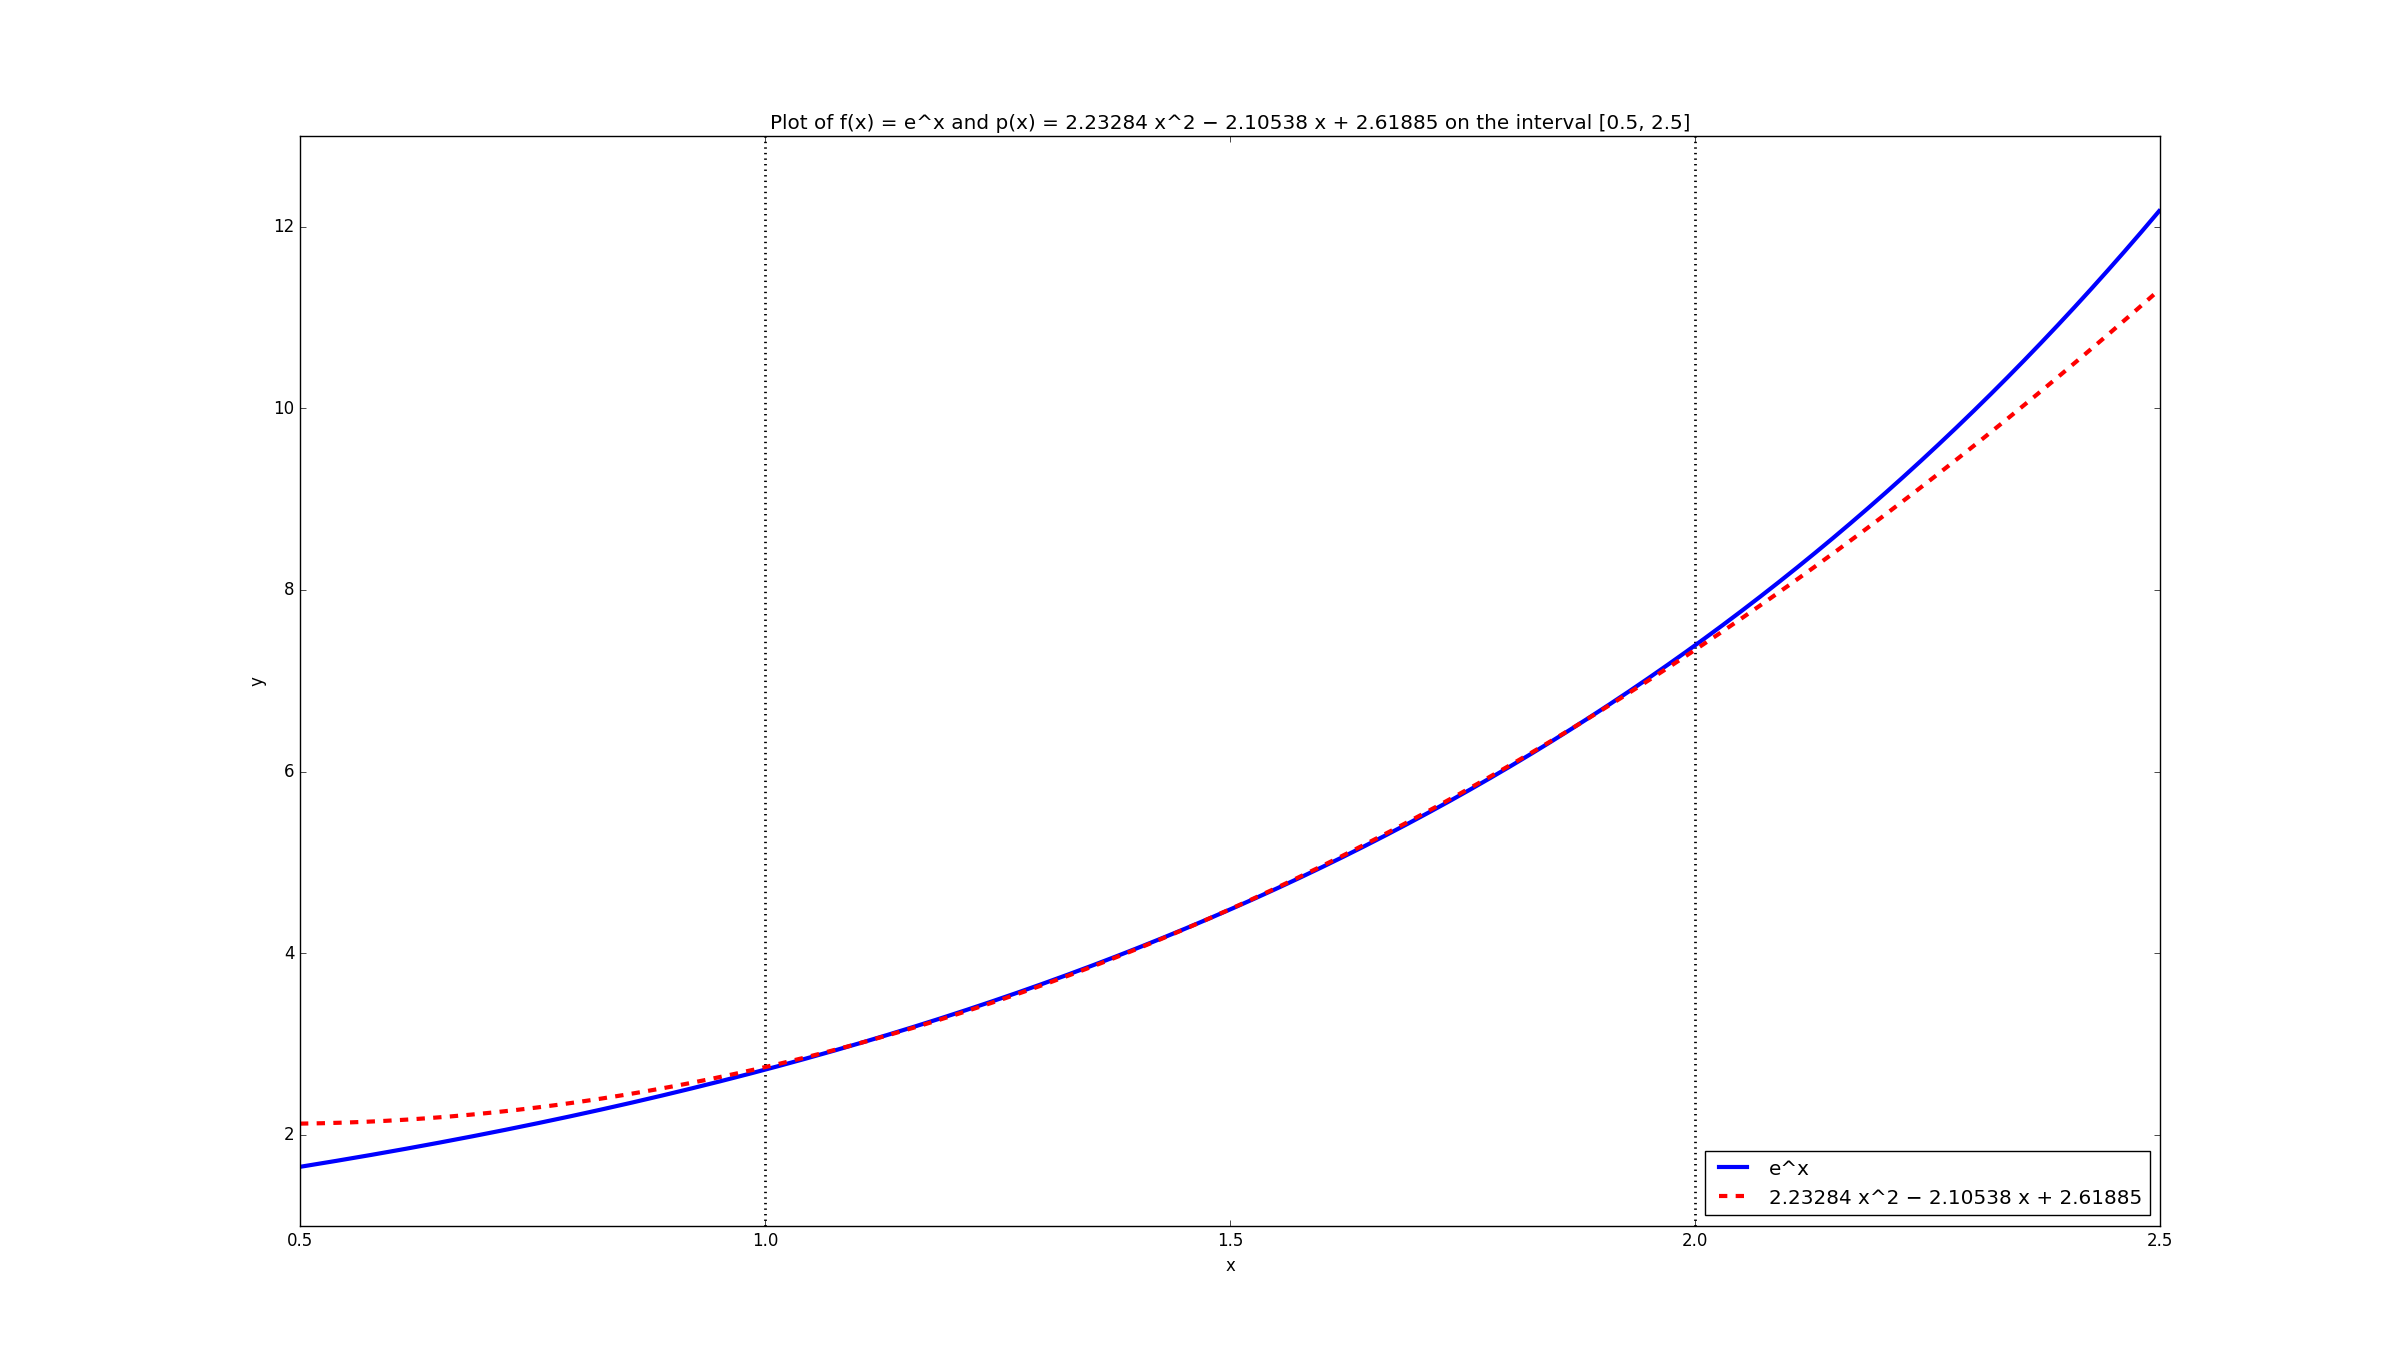
\includegraphics[trim={6cm, 0, 5cm, 2cm}, clip, width=\textwidth]{ortho_plot.png}
	\vspace{-10mm}
	\caption{Plot of $f(x) = e^x$ (solid line) and $p(x) = 2.23284 x^2 - 2.10538 x + 2.61885$ (dashed line), the polynomial constructed in 2 (a).}
	\label{Figure 1}
\end{figure}

% Stuff for wolfram alpha to simplify
(\frac{1}{4} n^2 + \frac{1}{4} n) (\frac{5}{4} n^2 + \frac{13}{4} n + \varepsilon) - n (\frac{5}{12} n^3 + \frac{9}{8} n^2 + \frac{17}{24} n + \delta)

(\frac{1}{4} n^2 + \frac{1}{4} n)^2 - n (\frac{1}{12} n^3 + \frac{1}{8} n^2 + \frac{1}{24} n)

% Incorrect work for #3
Hence $$\phi_0 (t) = \sqrt{1/2}, \ \ \ \phi_1 (t) = \sqrt{3/2} \ (t + 2), \ \ \ \text{and} \ \ \ \phi_2 (t) = \sqrt{5/8} \ (3t^2 + 12 t + 11).$$ Now by defining $f(t) = e^{t + 2}$ we have $$p_2 (t) = \langle f(t), \phi_0 \rangle \phi_0 + \langle f(t), \phi_1 \rangle \phi_1 + \langle f(t), \phi_2 \rangle \phi_2.$$ Since $$\langle f(t), \phi_0 \rangle = e^2 \sqrt{\frac{1}{2}} \int_{-1}^{1} e^t \approx 12.28050385,$$ $$\langle f(t), \phi_1 \rangle = e^2 \sqrt{\frac{3}{2}} \int_{-1}^{1} e^t (t + 2) = 2 e^3 \sqrt{\frac{3}{2}} \approx 49.19931667,$$ and $$\langle f(t), \phi_2 \rangle = e^2 \sqrt{\frac{5}{8}} \int_{-1}^{1} e^t (3t^2 + 12t + 11) = e^2 \left( 14 e - \frac{2}{e} \right) \sqrt{\frac{5}{8}} \approx 218.0081755$$ we have that 
\begin{align*}
p_2 (t) = 12.28050385 \sqrt{\frac{1}{2}} + 49.19931667 (t + 2) \sqrt{\frac{3}{2}} + 218.0081755 (3t^2 + 12 t + 11) \sqrt{\frac{5}{8}} \\
&= 
\end{align*}

% Some unused code
# Generate data set {(x_1, y_1), ..., (x_20, y_20)}
    for k in range(1, m + 1):
        # Initialize x_k = k/2
        x.append(k/2)

        # Initialize eps_k as a random number uniformly distributed in [-2, 2]
        epsilon = np.random.uniform(-2, 2)

        # Set y_k = 5x_k + 2 + eps_k
        y.append(5*k/2 + 2 + epsilon)
